\begin{figure}
	\centering
	\begin{minipage}{0.45\textwidth}
		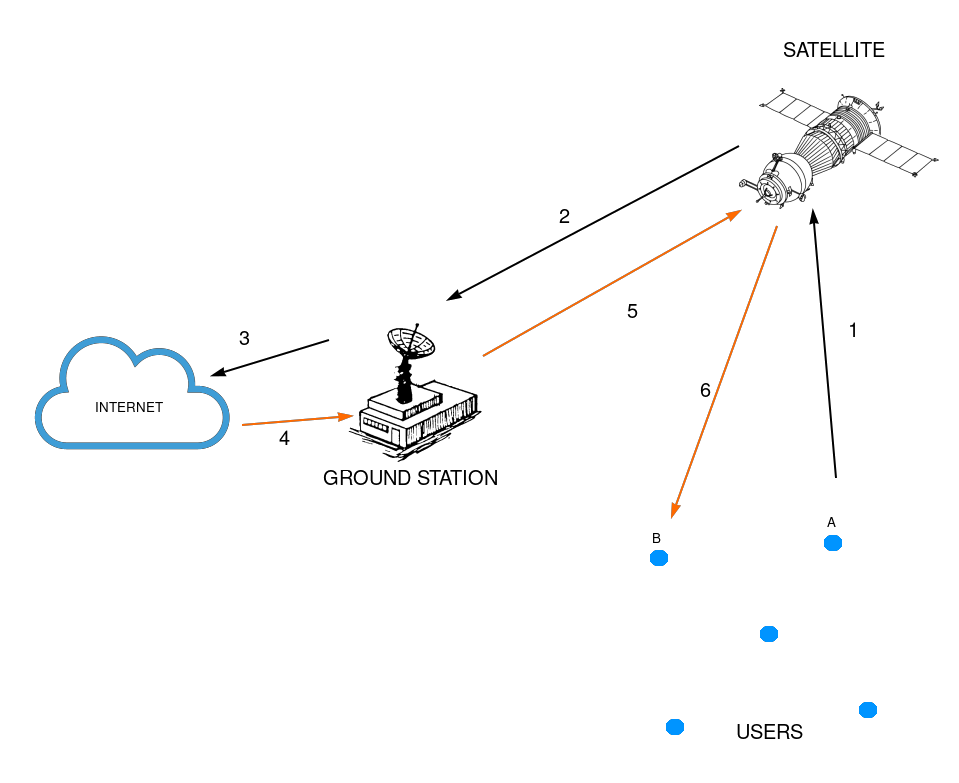
\includegraphics[width=\textwidth]{figures/System_topology_noBG.png}
		\caption{Scheme of the topology of the system.}
		\label{fig:topology}
	\end{minipage}\hspace{0.5cm}
	\begin{minipage}{0.45\textwidth}
		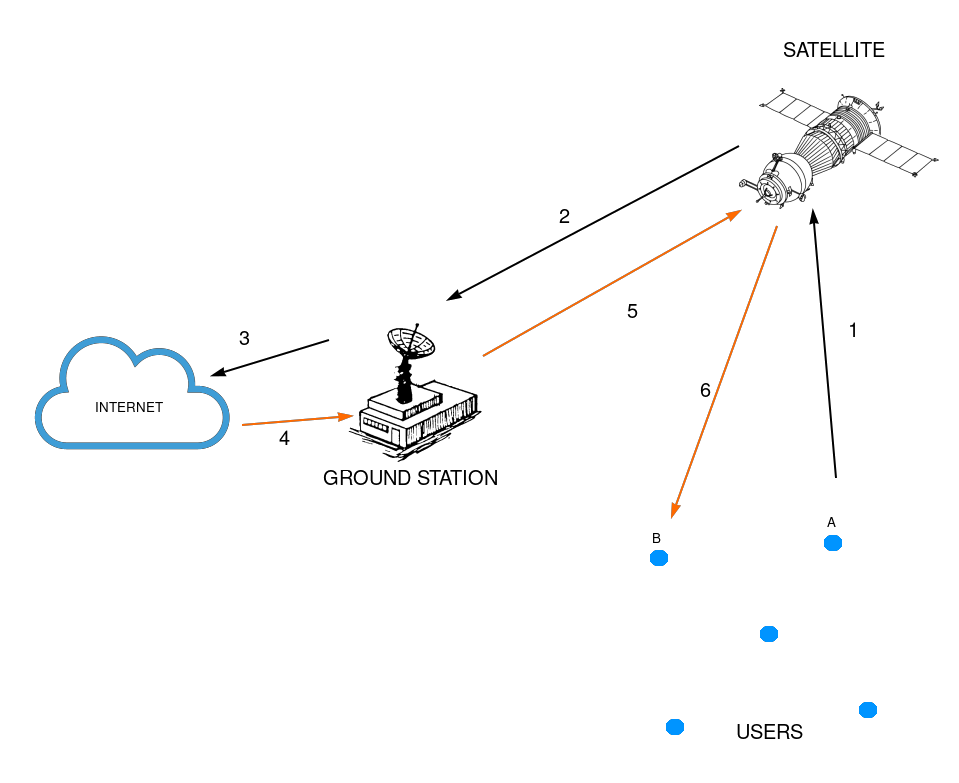
\includegraphics[width=\textwidth]{figures/System_topology_noBG.png}
		\caption{Typical communication path between an user A and an user B.}
		\label{fig:communication}
	\end{minipage}
\end{figure}

This project results from the necessity of having a good broadband coverage of polar
areas and the land areas of Northern Europe and Russia: this means the coverage of
latitudes over $60^\circ$.

The subjects interested in this kind of communication are
mostly industries involved in economic sector: they need a reliable communication system able to provide a service of 50 Mbps in download and 5 Mbps in upload.


The aim is to project a system able to provide a continuous, reliable and feasible communication service, maximizing the number of users allowed to access it over $60^\circ$
latitudes and minimizing the costs. To do that, services in narrowband communication using LEO satellites are not useful, since the broadband communication required is not feasible with this technology.

A simple representation of the system to be built is shown in \autoref{fig:topology} and a communication between two users is in \autoref{fig:communication}.

Typically, if a user A has to communicate with user B, it sends his packets to the satellite, with the recipient address in the header.
The satellite receives the packets and forwards them to the Ground Station that sends them to the proper application (Skype, Hangout, ...).
These packets are sent from the application to the Ground Station, that forwards them, through the satellite, to the recipient B.
